\section{Parallel projections}

Parallel projections are a type of graphical projection where all projection lines are parallel to each other, resulting in objects appearing the same size regardless of their distance from the observer. 
In parallel projections, the projection plane is positioned perpendicular to the line of sight, and there is no foreshortening or perspective distortion.

\subsection{Orthogonal projections}
Orthogonal projections are characterized by projecting onto planes that align with the $xy$, $yz$, or $zx$ planes, with the projection rays perpendicular to these planes. 
They find primary use in technical drawings, as segments of equal length parallel to an axis retain their identical properties.

It's important to recognize that each plane has two distinct projection directions, resulting in differing orderings of the $z$-component of normalized screen coordinates. 
This can sometimes produce entirely different images.

We'll initially focus on a projection plane corresponding to the $xy$-plane, which is perpendicular to the $z$-axis.
In this setup, visible objects possess negative values in their $z$ coordinate.

The screen boundaries naturally constrain the portion of the 3D world visible on a screen along the horizontal and vertical axes. 
However, it's also necessary to limit the range of a scene along the depth axis for several reasons:
\begin{enumerate}
    \item Prevent displaying objects behind the observer.
    \item Avoid showing objects that are excessively distant from the viewer's perspective.
    \item Enable the $z$-axis of the normalized screen coordinates to be confined within the $0$ to $+1$ range.
\end{enumerate}
These constraints define two planes:
\begin{itemize}
    \item The plane with the closest $z$-component (maximum signed value, minimum absolute value) is termed the near plane.
    \item The one with the farthest $z$-component (minimum signed value, maximum absolute value) is referred to as the far plane.
\end{itemize}
After projection, only points contained within the box bounded by the left, right, top, and bottom screen borders, as well as the near and far planes along the depth axis, can be visualized.
Normalized Screen Coordinates are defined such that the near plane, the left side, and the bottom side of the screen are projected to $z_n=0$, $x_l=-1$, and $y_t=-1$, respectively. 
Conversely, the far plane, the right side, and the top side are projected to $z_f=1$, $x_r=1$, and $y_b=1$, respectively.

\paragraph*{Orthogonal projection matrix}
Orthogonal projections can be implemented by normalizing the $x, y, z$ coordinates of the projection box within the ranges $(-1,1)$, $(-1,1)$, and $(0,1)$ respectively. 
This normalization process, starting from a valid coordinate, can be achieved by multiplying with a suitable matrix.
In particular, we define the projection matrix, $P_{ort}$, as the matrix that, when multiplied with a world coordinate $p_W$, computes the corresponding normalized screen coordinate $p_N$: 
\[P_N=P_{ort}\cdot P_W\]
To obtain normalized coordinates, we must determine the coordinates of the screen borders in 3D space.
We denote $l$ and $r$ as the x-coordinates in 3D space corresponding to locations displayed on the left and right borders of the screen. 
Anything to the left of $l$ will be excluded from the screen, and nothing to the right of $r$ will be visualized. 
Similarly, we use $t$ and $b$ for the $y$-coordinates of the top and bottom borders of the screen in 3D space.
$P_{ort}$
We also denote $-n$ and $-f$ as the $z$-coordinates of the near and far planes in 3D space. 
Since the $z$-axis is oriented opposite to the viewer's perspective, positive distances $n$ and $f$ are generally preferred over negative coordinates where the two planes intersect.

The orthogonal projection matrix $P_{ort}$ is computed in three steps. 
First, we translate the center of the projection box to the near plane at the origin using a translation $T_{ort}$:
\[T_{ort}=\begin{bmatrix}
    1 & 0 & 0 & -\frac{r+l}{2} \\ 
    0 & 1 & 0 & -\frac{t+b}{2} \\ 
    0 & 0 & 1 & -(-n) \\ 
    0 & 0 & 0 & 1 
\end{bmatrix}\]
The second step involves normalizing the coordinates between $-1$ and $1$ (for the $x$-axis and $y$-axis) or 0 and 1 (for the $z$-axis) through a scale transformation $S_{ort}$:
\[S_{ort}=\begin{bmatrix}
    \frac{2}{r-l} & 0 & 0 & 0 \\ 
    0 & \frac{2}{t-b} & 0 & 0 \\ 
    0 & 0 & \frac{1}{f-n} & 0 \\ 
    0 & 0 & 0 & 1 
\end{bmatrix}\]
The last step corrects the direction of the axes with the mirror matrix $M_{ort}$, by inverting the $y$-axis and $z$-axis:
\[M_{ort}=\begin{bmatrix}
    1 & 0 & 0 & 0 \\ 
    0 & -1 & 0 & 0 \\ 
    0 & 0 & -1 & 0 \\ 
    0 & 0 & 0 & 1 
\end{bmatrix}\]
By applying the composition of transformations, we can define the orthogonal projection matrix $P_{ort}$ as follows:
\[M_{ort}=M_{ort}\cdot S_{ort} \cdot T_{ort}=\begin{bmatrix}
    \frac{2}{r-l} & 0 & 0 & \frac{r+l}{l-r} \\ 
    0 & \frac{2}{b-t} & 0 & \frac{t+b}{t-b} \\ 
    0 & 0 & \frac{1}{n-f} & \frac{n}{n-f} \\ 
    0 & 0 & 0 & 1 
\end{bmatrix}\]

\subsection{Aspect ratio}
The ratio between the horizontal and vertical dimensions of the physical screen is known as the aspect ratio: 
\[a=\dfrac{D_x}{D_y}\]
In this definition, the measures for the horizontal and vertical sizes, $D_x$ and $D_y$, are specified in metric units rather than pixels. 
When pixels are square, both metric units and pixels yield the same outcome. 
However, if pixels are not square, only the actual display proportions can ensure images are not distorted.

Normalized screen coordinates do not incorporate the aspect ratio. 
Instead, the projection matrix adjusts for this factor, appropriately scaling the images to ensure they appear with the correct proportions.

To generate images with accurate proportions, the values of $l$, $r$, $t$, and $b$ must be consistent with the aspect ratio $a$ of the monitor: 
\[a=\dfrac{r-l}{t-b}\rightarrow r-l=a\cdot (t-b)\]
In many cases, the projection box is centered at the origin both horizontally and vertically. 
When this occurs, only the half-width of the box $w$, the near plane $n$, the far plane $f$, and the aspect ratio $a$ are required.
\[\begin{cases}
    l=-w \\
    r=w \\
    t=\frac{w}{a} \\
    b=-\frac{w}{a}
\end{cases}\]
As a result the transformation matrix becomes: 
\[P_{ort}=\begin{bmatrix}
    \frac{1}{w} & 0 & 0 & 0 \\ 
    0 & -\frac{a}{w} & 0 & 0 \\ 
    0 & 0 & \frac{1}{n-f} & \frac{n}{n-f} \\ 
    0 & 0 & 0 & 1 
\end{bmatrix}\]

For orthogonal projections where the near plane is positioned at $n=0$, the projection matrix can be further simplified into a non-uniform scaling matrix with factors $S(\frac{1}{w}, -\frac{a}{w}, -\frac{1}{f})$:
\[P_{ort}=\begin{bmatrix}
    \frac{1}{w} & 0 & 0 & 0 \\ 
    0 & -\frac{a}{w} & 0 & 0 \\ 
    0 & 0 & -\frac{1}{f} & 0 \\ 
    0 & 0 & 0 & 1 
\end{bmatrix}\]

While World Coordinates are represented using Homogeneous coordinates, Normalized Screen Coordinates are Cartesian coordinates. 
Therefore, a conversion procedure from one system to the other must be performed (division of the first three components by the fourth).

For parallel projection, since it's implemented using a sequence of conventional transform matrices, the last element of $P_N$ is always one. 
This implies that Normalized Screen Coordinates can be obtained by simply discarding the fourth element of the vector resulting from the product of the homogeneous coordinates with the projection matrix.

\paragraph*{Orthogonal projections in GLM}
GLM gives the \texttt{ortho()} function to compute the orthographic projection matrix specifying the boundaries:
\begin{verbatim}
glm::mat4 Port = glm::ortho(l, r, b, t, n, f);
\end{verbatim}
Here, $l$, $r$, $b$, $t$, $n$, $f$ are the positions in world coordinates respectively of the left, right, bottom, top, near and far boundaries of the visible region.
Keep however in mind that such procedure was created for the Normalized Screen Coordinates conventions of OpenGL, and the result will not work correctly in Vulkan without further modifications.
In order to make it work, the following additions must be done: 
\begin{verbatim}
#define GLM_FORCE_DEPTH_ZERO_TO_ONE    

Port = glm::scale(glm::mat4(1.0f), glm::vec3(1,-1,1)) * 
                  glm::ortho(l, r, b, t, n, f);
\end{verbatim}

\subsection{Axonometric projections}
Many objects conform to shapes that align with the sides of a box. 
In parallel projections, faces perpendicular to the projection plane are concealed. When a cube is aligned with the three main axes, it presents as a square, restricting depth perception. 
Axonometric projections resolve this constraint by simultaneously displaying all cube faces.
Axonometric projections enable the viewing of all faces of box-shaped objects by either rotating the projection plane relative to the three main axes or by adjusting the angle of the projection plane so that it is no longer perpendicular to the projection rays.

\paragraph*{Orthographic projections}
Orthographic projections are a type of axonometric projection where rays are perpendicular to the projection plane.
The principal orthographic axonometric projections include:
\begin{itemize}
    \item \textit{Isometric}: the three axes are oriented at angles of $120^\circ$ from one another.
        Segments of equal lengths aligned parallel to the main axis in three-dimensional space maintain equal lengths when projected onto a two-dimensional plane.
        Isometric projections are achieved by first rotating $\pm 45^\circ$ around the $y$-axis, followed by a rotation of $\pm 35.26^\circ$ around the $x$-axis, before applying the parallel projection as previously described.
        It's worth noting that in this scenario, the projection matrix needs to be specified with the half-width and the aspect ratio, as the box's borders displayed on the screen are no longer aligned with the main axis. 
        \[\begin{bmatrix}
            \frac{1}{w} & 0 & 0 & 0 \\ 
            0 & -\frac{a}{w} & 0 & 0 \\ 
            0 & 0 & \frac{1}{n-f} & \frac{n}{n-f} \\ 
            0 & 0 & 0 & 1 
        \end{bmatrix}\begin{bmatrix}
            1 & 0 & 0 & 0 \\ 
            0 & \cos(35.26^\circ) & \sin(35.26^\circ) & 0 \\ 
            0 & -\sin(35.26^\circ) & \cos(35.26^\circ) & 0 \\ 
            0 & 0 & 0 & 1 
        \end{bmatrix}\begin{bmatrix}
            \cos(45^\circ) & 0 & \sin(45^\circ) & 0 \\ 
            0 & 1 & 0 & 0 \\ 
            -\sin(45^\circ) & 0 & \cos(45^\circ) & 0 \\ 
            0 & 0 & 0 & 1 
        \end{bmatrix}\]
        The rotations around the $x$ and $y$ axes, with their respective signs, yield four distinct yet equally valid axonometric projections.
    \item \textit{Dimetric}: in dimetric projection, distinct units are used for the $x$ and $z$-axes compared to the $y$-axis. 
        Its popularity in the 1980s stemmed from its simplicity in implementation through integer arithmetic.
        Even today, dimetric projection remains prevalent in retro-style games and applications.
        To obtain dimetric projections, a rotation of $\pm 45^\circ$ around the $y$-axis is first applied, followed by an arbitrary rotation $\alpha$ around the $x$-axis, before executing the basic parallel projection:
        \[\begin{bmatrix}
            \frac{1}{w} & 0 & 0 & 0 \\ 
            0 & -\frac{a}{w} & 0 & 0 \\ 
            0 & 0 & \frac{1}{n-f} & \frac{n}{n-f} \\ 
            0 & 0 & 0 & 1 
        \end{bmatrix}\begin{bmatrix}
            1 & 0 & 0 & 0 \\ 
            0 & \cos(\alpha) & \sin(\alpha) & 0 \\ 
            0 & -\sin(\alpha) & \cos(\alpha) & 0 \\ 
            0 & 0 & 0 & 1 
        \end{bmatrix}\begin{bmatrix}
            \cos(45^\circ) & 0 & \sin(45^\circ) & 0 \\ 
            0 & 1 & 0 & 0 \\ 
            -\sin(45^\circ) & 0 & \cos(45^\circ) & 0 \\ 
            0 & 0 & 0 & 1 
        \end{bmatrix}\]
    \item \textit{Trimetric}: in trimetric projection, each axis has a different unit.
    To obtain trimetric projections, an arbitrary rotation $\beta$ around the $y$-axis is first applied, followed by an arbitrary rotation $\alpha$ around the $x$-axis, before executing the parallel projection:
        \[\begin{bmatrix}
            \frac{1}{w} & 0 & 0 & 0 \\ 
            0 & -\frac{a}{w} & 0 & 0 \\ 
            0 & 0 & \frac{1}{n-f} & \frac{n}{n-f} \\ 
            0 & 0 & 0 & 1 
        \end{bmatrix}\begin{bmatrix}
            1 & 0 & 0 & 0 \\ 
            0 & \cos(\alpha) & \sin(\alpha) & 0 \\ 
            0 & -\sin(\alpha) & \cos(\alpha) & 0 \\ 
            0 & 0 & 0 & 1 
        \end{bmatrix}\begin{bmatrix}
            \cos(\beta) & 0 & \sin(\beta) & 0 \\ 
            0 & 1 & 0 & 0 \\ 
            -\sin(\beta) & 0 & \cos(\beta) & 0 \\ 
            0 & 0 & 0 & 1 
        \end{bmatrix}\]
\end{itemize}
\begin{figure}[H]
    \centering
    \begin{subfigure}{0.32\textwidth}
        \centering
        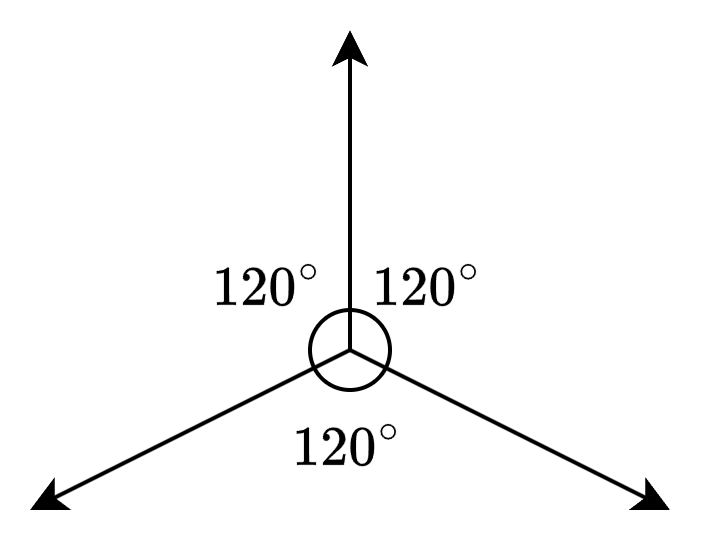
\includegraphics[width=0.75\linewidth]{images/iso.png} 
        \caption{Isometric}
    \end{subfigure}
    \begin{subfigure}{0.32\textwidth}
        \centering
        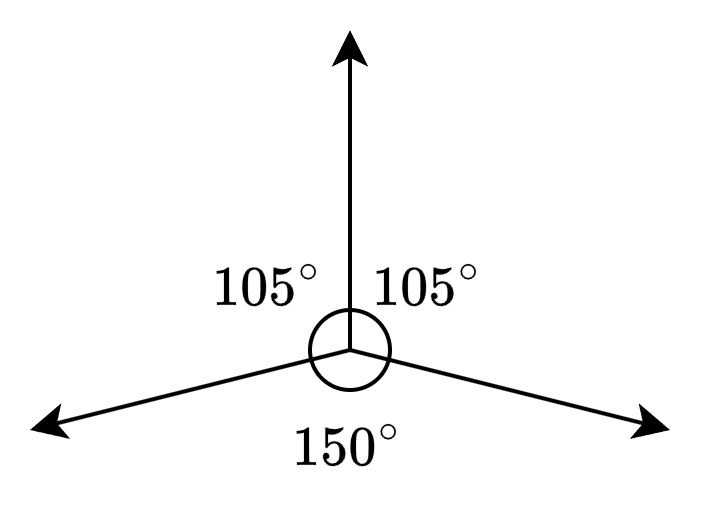
\includegraphics[width=0.75\linewidth]{images/dim.png}
        \caption{Dimetric}
    \end{subfigure}
    \begin{subfigure}{0.32\textwidth}
        \centering
        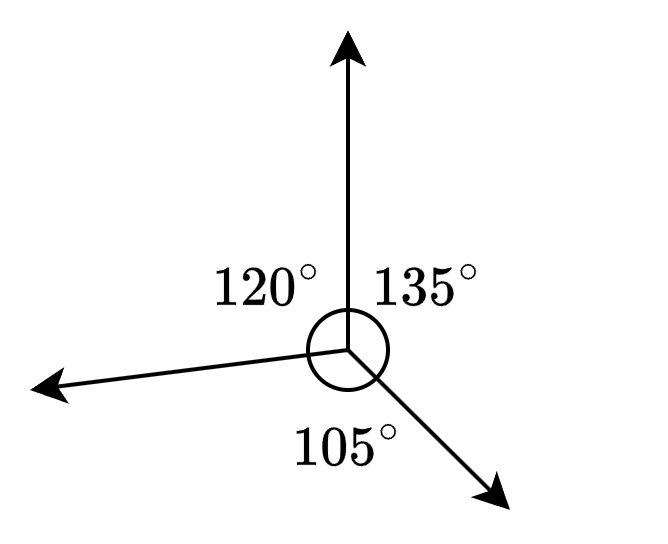
\includegraphics[width=0.75\linewidth]{images/tri.png} 
        \caption{Trimetric}
    \end{subfigure}
    \caption{Orthographic projections}
\end{figure}
A fundamental characteristic of axonometric projections is that they preserve the upward axis (the $y$-axis in our context) parallel to the vertical orientation of the screen.

\subsection{Oblique projections}
In oblique projections, rays are parallel but oblique in relation to the projection plane. 
Consequently, two of the three axes ($x$ and $y$) run parallel to the screen, while the third axis ($z$) is inclined at an angle to the other two.
The $z$-axis is commonly angled at $45^\circ$, $30^\circ$, or $60^\circ$, and it can be oriented in either direction.
The length of the $z$-axis can either match that of the other two axes or be halved. 
If the length is preserved, the projection is termed Cavalier; otherwise, it's referred to as Cabinet.

Oblique projections, valued for their simplicity in implementation using only integer arithmetic, found utility in some arcade and PC games.

These projections are achieved by applying a shear along the $z$-axis before the orthogonal projection:
\[\begin{bmatrix}
    \frac{1}{w} & 0 & 0 & 0 \\ 
    0 & -\frac{a}{w} & 0 & 0 \\ 
    0 & 0 & \frac{1}{n-f} & \frac{n}{n-f} \\ 
    0 & 0 & 0 & 1 
\end{bmatrix}\begin{bmatrix}
    1 & 0 & -\rho\cos(\alpha) & 0 \\ 
    0 & 1 & -\rho\sin(\alpha) & 0 \\ 
    0 & 0 & 1 & 0 \\ 
    0 & 0 & 0 & 1 
\end{bmatrix}\]
The shear factor determines the projection angle and whether it will be Cavalier or Cabinet. 
Specifically, it can be defined with respect to the axis angle, denoted as $\alpha$, and the corresponding reduction factor, denoted as $\rho$:
\begin{itemize}
    \item Cavalier: $\alpha=45^\circ$, $\rho=1$.
    \item Cabinet: $\alpha=45^\circ$, $\rho=0.5$.
\end{itemize}